\documentclass[../PiTest.tex]{subfiles}

\begin{document}

\section{Project definition}

    The project definition will be split in two sections, describing the server and on the client.

    \subsection{Server}
    The server application, from now on \pitest, is installed on the Operating System of the board and needs NodeJS to work.

    \subsubsection{Class diagram}
    The following is an high level diagram of the architecture of \pitest.
    
    \begin{figure}[!h]
        \centering
        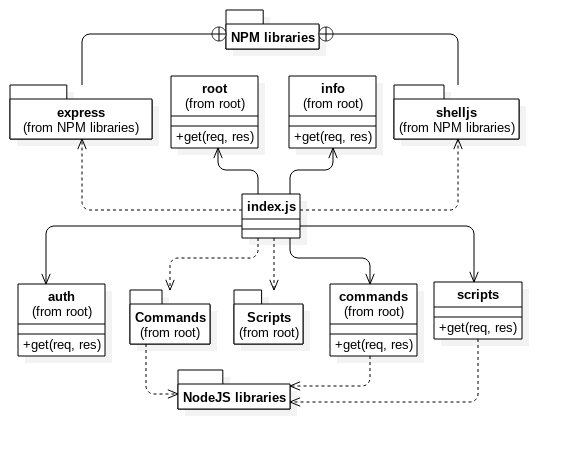
\includegraphics[width=\textwidth+1cm, height=10cm, keepaspectratio]{\detokenize{UML/png/Model__High level server diagram_1.png}}
        \caption{High level architectural diagram}
    \end{figure}

    \subsubsection{Modules}

    \paragraph{index.js}
    This is the main file of the application, it creates an Express app and loads all the routes of the web app.
    
    \paragraph{root}
    Defines the behaviour of the root page (\texttt{/}), it's purpose is to respond with a custom welcome message.

    \paragraph{info}
    Defines the behaviour of the root \texttt{/info}, it gives information about the server, as its name, version and author; it requires authentication using a valid token.

    \paragraph{auth}
    Defines the behaviour of the root \texttt{/auth}, it's used to authenticate the user and requires a valid token.

    \paragraph{commands}
    Defines the behaviour of the root \texttt{/commands}, it's used to list to the user the possible commands and all their parameters; it requires authentication using a valid token.

    \paragraph{scripts}
    Defines GTE behaviour of the root \texttt{/scripts}, it's used to list to the user the possible scripts and all their parameters; it requires authentication using a valid token.

    \subsubsection{Dependencies}
    Since the necessity of a solid code base from which extend the application, I have chosen to use some common libraries, both from the standard NodeJS ones and from NPM modules.

    \paragraph{fs}
    It's a NodeJS standard library which allows to read files on the file system.

    \paragraph{events}
    It's a NodeJS standard library which allows to use the event system.

    \paragraph{express}
    It's a \npm library which allows to generate a complete web server; it's used as a base for the REST API. (\url{https://www.npmjs.com/package/express})

    \paragraph{shelljs}
    It's a \npm library which allows to execute shell commands on the host in bot synchronous and asynchronous ways. It's used to call the host executables from the server.

    \clearpage

    \subsection{Low level UML diagram}
    \begin{figure}[!h]
        \centering
        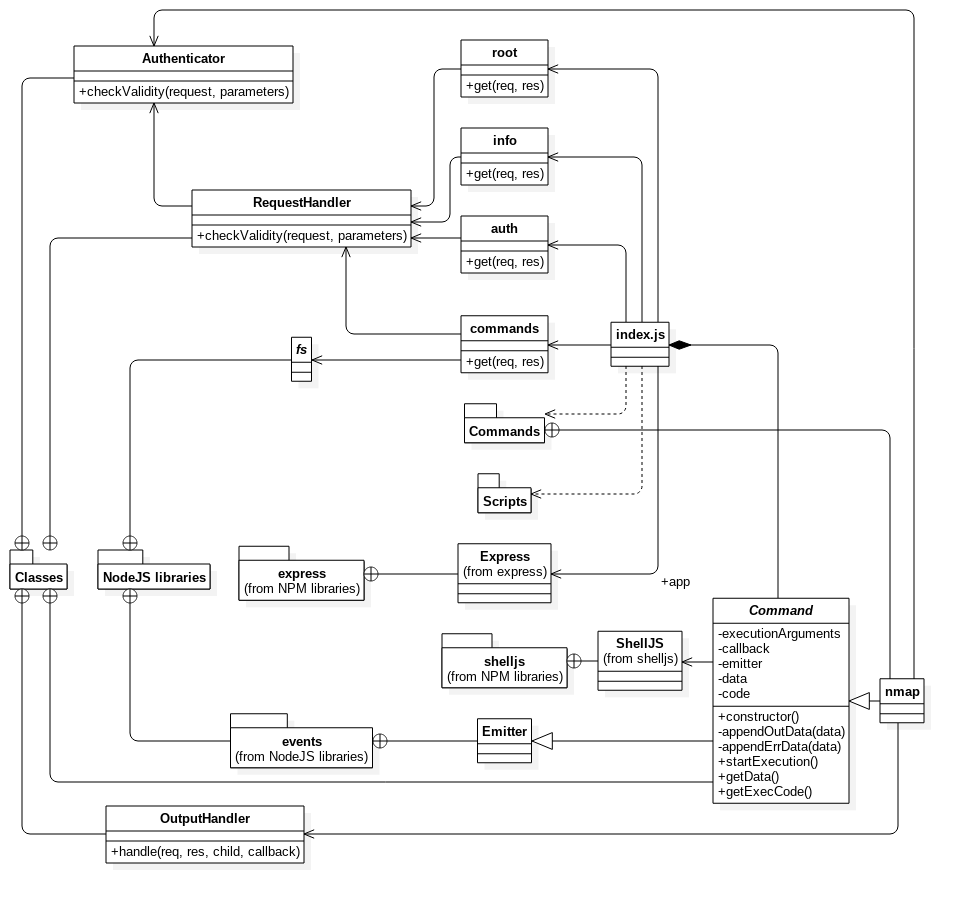
\includegraphics[width=\textwidth+1cm, keepaspectratio]{\detokenize{UML/png/Model__Low level server diagram_0.png}}
        \caption{Low level UML diagram of PiTest}
    \end{figure}

    \subsection{Commands and scripts}
    To easily control the execution of commands and scripts I have chosen to create two respective wrapper classes, which contain all the information needed for the execution, have a simple interface to start the execution and retrieve the result with a callback. Also, every time there is an output, both on \texttt{STDERR} or \texttt{STDOUT} from the shell, an event, containing the relevant data, is created.

\end{document}